\section{Modular approaches in manipulation}
\label{cha4:sec2}


We have briefly introduced our method in the previous section and
justified our design decisions in the light of related literature.  In
this section we present our method for modularizing human
demonstrations of manipulation tasks. Our goal is to acquire a modular
control policy for an object manipulation task from human
demonstration. To this end, we take a three-step approach:
\begin{enumerate}
\item Human demonstration of a task in several different contexts  (Section~\ref{cha4:sec2:demo}).
\item Extraction and modular decomposition of human control strategies
  for different contexts, building multiple internal models(Section~\ref{cha4:sec2:learn}).
\item Robot control using the integrated modules to compute motor
  commands (Section~\ref{cha4:sec2:control}).
\end{enumerate}

Figure~\ref{fig:overview} shows an overview of our framework.

\begin{figure}
  \centering
   \includegraphics[width=15cm]{./fig_cha4/overview3.pdf}
  \caption{ \scriptsize{System overview. Our system takes a
       three-step approach. 1) A human demonstrates a task in a
       variety of contexts. In the opening-bottle-cap experiment, the
       demonstrations are done with different bottles and caps. The
       object-level exerted forces and torque, and the the object's
       movements are used for training. 2) Clustering is run over the data from the human control
       strategies. Each cluster is then modeled as one module. 3) The
       multiple modules are integrated to compute motor commands to
       control a robot performing the same task in similar contexts}
  \label{fig:overview}
}
\label{fig:demo}
\end{figure}

\subsection{Human demonstrating tasks involving direct contact with objects}
\label{cha4:sec2:demo}


\begin{figure*}
  \centering
    \subfloat[\scriptsize{Optitrack markers attaching to a cap}] {\includegraphics[height=4cm]{./fig_cha4/marker2.jpg}}
    \subfloat[\scriptsize{Force torque sensor}] {\includegraphics[height=4cm]{./fig_cha4/Nano25-E.jpg}}
    \subfloat[\scriptsize{Texscan tactile sensors mounting to a glove}] {\includegraphics[height=4cm]{./fig_cha4/texscan2.jpg}}
    \caption{\scriptsize{Sensors used in the human demonstration of opening a bottle cap task.}}
  \label{fig:devices}
\end{figure*}

%Learning manipulation tasks is one of the main application of this approach. The physical properties of a manipulation task is hard to express analytically, and as a result the control strategy is hard to derive. Modeling expert's demonstration of strategies has been used as an alternative to the analytical solution.

The first step is to demonstrate a task to a robot. Demonstration-based learning has been extensively studied~\citep{calinon2007learning,dillmann2004teaching,kulic2012incremental}
as a promising approach for building robot
intelligence. %It is essential for the tasks that analytical expression of the system is hard to derive.
Learning manipulation tasks is one of the main application of this
approach. The physical properties of a manipulation task is hard to
express analytically, and as a result the control strategy is hard to derive. Modeling an expert's demonstration
of strategies has been used as an alternative to fully analytical
solutions.In previous studies, two major forms of demonstration are used in teaching manipulation tasks: kinematics teaching and tele-operation.

\paragraph{Kinematics teaching} ~\\
% ===== Why not kinematics approach? =====
In kinesthetic
teaching, a human directly contacts the robot and guides the robot's
movements to accomplish a
task~\citep{korkinof2013online,pais2014encoding,pastor2011skill,Miao2014}. The
trajectory of movements and contact force are recorded by the robot's
sensors.
% ===== Why not kinesthetic approach? =====
This method is simple and effective, but it is limited in the number
of controllable end effectors. %JJB is this right?
While a manipulation task usually involves multi-finger movement, a
human can only operate one finger with each hand and hence
two fingers simultaneously at most. Hence kinesthetic teaching is not feasible for demonstrating multi-finger tasks.

\paragraph{Tele-operation teaching} ~\\
To control multi-finger hands,
some researchers use
tele-operation~\citep{bernardino2013precision,kondo2008recognition,Fischer1998}.
This usually relies on data gloves or other motion-capture systems, which
sense the human hand and arm motions. The human motion is mapped to
the robot's to generate motions in the robot in real time, allowing
the robot to record its own interactions with the environment.
In fine manipulation tasks, the robot platforms are usually restricted
to anthropomorphic hands for better mapping.
Neither kinesthetic teaching nor
tele-operation method provides direct force
feedback to the human demonstrator during manipulation. With only visual feedback,
it is difficult for the human to conduct manipulation naturally.

\paragraph{Human direct demonstration} ~\\
Another approach involves the human demonstrating manipulation tasks
with their own bodies, rather than directing the
robot~\citep{asfour2008imitation}. With direct interaction with the
object, the human demonstrator is able to perform the task most
naturally and with a more delicate control strategy. However, the task
information captured from these human demonstrations must then be
transferred to robots. This involves the problem of creating a mapping
between the motions of a human and those of a robot, a problem known
as the correspondence problem \citep{Nehaniv02}.
Various methods for mapping between human and
robot have been
proposed~\citep{hueser2006learning,asfour2008imitation,do2011towards}. These may be augmented with correction by humans~\citep{calinon2007incremental,sauser2011iterative,romano2011human}
and by self-correction via learning~\citep{bidan2013robio}. In general, the effective transfer of human skills to robots skills remains a challenge.

Our proposed method derives from this last class of demonstrations.
We allow the subject to perform a manipulation task directly on an object and experience natural feedback. Our contribution is to
encode the strategy in a way that can then be
easily transferred to any robot platform. In our task demonstration, a human wears tactile sensors mounted on a dataglove, and directly
interacts with objects. In this way, human demonstrators have direct cutaneous and kinaesthetic feedback, which is desirable for good manipulation demonstration. To make the information embedded in the demonstration easily transferable to robots, the demonstration is recorded and expressed
from an object-centric viewpoint.


%============= Object Centric =============
\paragraph{Object centric representation} ~\\
The object-centric
viewpoint~\citep{okamura2000overview,jain2013improving,Miao2014}
centers the representation of the manipulation task on the manipulated object, rather than on the robot. This suggests that the goal of a manipulation task is to produce a desired
object movement rather than a robot end-effector movement. This makes sense also in the learning from human demonstration approach: humans may use different postures to accomplish a manipulation task and hence their motion or posture might be different but the effect on the object is the same. What the robot needs to imitate is the effect on the object but not the human posture.
Hence our approach takes this principle and learns a control strategy for
producing a desired object behavior. The demonstrated strategy expressed from the object perspective can then be transferred to a robot platform by converting the exerted force to robot joint torque.
With the object centric viewpoint the manipulation problem is simplified: we transfer from a problem of controlling multi-finger (multi-end-effector) and its interaction with the environment to controlling an object behavior.

Based on the object-centric principle, we collect the object's trajectory and the force driving it. We collected this data by a vision-based motion-capture system,
force-torque sensor and wearable haptic
devices. Figure.~\ref{fig:devices} shows a few of the sensors we used
in the opening-bottle-caps task. The representation of the data will be explained in Section~\ref{cha4:sec2:learn:objectlevel}


% ======= demonstrate in different context   =======
\paragraph{Demonstrations in different task contexts}  ~\\
In the demonstrations, the demonstrator performs a task a number of
times to generate enough data to reliably capture its key features.
The demonstrator also performs the task under a variety of conditions, e.g. a range of friction conditions, in order to explore how humans adapt to different task contexts. These different configurations must be chosen to cover a wide range.
For example, in a opening-bottle-cap task, the demonstration of opening
the tightest bottle within the capability of the learner is
included. These wide range demonstrations are then used to learn a
multiple module model.

\subsection{Learning a Multiple-Module Model}
\label{cha4:sec2:learn}
Here we detail our modeling method, explaining how we model the human manipulation strategy.  This requires determining the number of modules to represent a task strategy, learning the internal models for driving each
module, and determining how to integrate the output of the modules.

% Our approach: modular approach
The excellent ability of humans to manipulate different objects in different contexts and to quickly adapt to changes of context suggest that our central nervous system (CNS) maintains multiple internal models of outside environments, rather than a single internal model that adapts to new environment~\cite{neilson1985acquisition}.
Inspired by this, we take a modular approach to model the human adaptive control strategy. More specifically, we take the paradigm of MOSAIC~\cite{haruno2001mosaic} that we introduce in Section~\ref{cha2:sec3:cognitive}.

%MOSAIC
The system of MOSAIC is constituted by multiple parallel modules. Each module has three components: a forward model, an inverse model and a responsibility factor (RF). The forward model is responsible for estimating the task context in real time, and the inverse model is used to generate appropriate motor commands for the context. These two models are connected by the RF. The task context estimated by the forward model is compared with the actual current task context.
The RF of each module is computed according to the similarity between the predicted context and the actual context: the more accurate the forward model predicts, the higher the RF is (detailed in Section~\ref{cha4:sec2:control:rf}). The RF's of all modules are computed and then normalized.
The inverse models are weighed by their normalized RF. The final motor command is the linear combination of the commands generated by each inverse models. With this mechanism, the modules best predicting the current task context take most responsibility in the final motor command. Figure~\ref{fig:control} sketches the work flow of this system. %Though this model has raised concerns in the neuroscience community, it is not widely used in robot control.

We take this paradigm, and model our internal models using GMM. Training GMM with the Expectation Maximization algorithm (EM), we estimate the optimal values of the model parameters. Compared to the early work~\cite{wolpert1998multiple} which use Neural Networks and have to manually tune the variance of each forward model, GMM has the advantage of automatically computing the all the model parameters. Later work~\cite{haruno2001mosaic} fixes the hand tuning problem by modelling with a Hidden Markov Model (HMM) and optimizing the model with EM. With this method the forward models are assumed to be linear. In our approach, GMM allows a non-linear system to be modelled. Fig.~\ref{fig:control} illustrates the workflow of our approach. Compared to the switching modular method~\cite{narendra1997adaptive}, i.e. only one module will be activated and used to generate motor command, the linear combination of the modules requires a smaller number of modules to approximate the system dynamics.

In some tasks the forward model and inverse model are united into a single model~\cite{petkos2006learning}. For that particular task the action ($a_t$) taking the current task state ($s_t$) to the desired task state ($s_{t+1}$) is always unique. However, in many cases this mapping is not unique and hence the inverse model has to include extra variables in order to resolve the non-uniqueness. In our approach we build the forward and inverse models separately.
%However this model does not provide a method to find out number of models needed in tasks. %and the inverse model represented by the joint distribution will potentially produce an invalid command that average all possible solutions.

Despite the many applications and discussions of the modular approach, how to systematically modularize the control strategy presented during the human demonstration, i.e. how to determine the number of modules and build an appropriate model for each module, still remains an open problem. We tackle this problem with a data driven approach. We cluster the demonstration data with a hierarchical approach and model each cluster as a pair of forward and inverse models. This solution can be applied to modularize many manipulation tasks. A similar clustering method has been applied to group and build tree structures of human motion pattern primitives~\cite{kulic2008incremental}. To cluster the motion primitives, a high value and a low value of the cut off parameter are tested to evaluate the trade off effect between facilitating quick tree formation and introducing misclassification. In our approach, the cut off parameter is determined by the variance of the data and hence avoids this step. This provide us with a proper grouping of the data which can then generate proper motor commands for control. To the best of our knowledge, our work is the first realization of the modular approach in learning an object manipulation task with a real robot.

%
%
%Scientist has long been fascinated by human adaptive motor control ability and wondering the mechanism of it. One of the most evidently supported hypothesis is the multiple model~\cite{neilson1985acquisition}. %~\cite{haruno2001mosaic}



\subsubsection{Object centric manipulation strategy}
\label{cha4:sec2:learn:objectlevel}


As mentioned in Section~\ref{cha4:sec2:demo}, one of the challenges in imitation learning is the mapping problem, i.e. how to map the teacher's motions to the robot's motions so that they produce the same effects. This mapping becomes more difficult for object manipulation tasks, the goal of which is to deliver the object from the current state to a desired state. During this process the movement of the manipulator is bounded not only by its own kinematic constraints but also bounded by by the movement of the object. The object centric approach we use here get around this problem by directly learning the manipulated object behavior.

%It is more important to imitate how humans apply forces to achieve an object's desired movement, than to imitate the human limb movement. Therefore we take an ``object centric approach"~\cite{okamura2000overview}, where the control policy is taken from the object's perspective.

The object-centric approach means that our model encodes a force and
torque profile rather than the end effector movement trajectory.  The
imitation-learning objective here is not to find a policy for the end
effector movement but to find a policy that maps force and torque
to object movements. This policy allows the robot to efficiently
acquire new behaviors to accomplish the
task. %Different robots move differently to achieve the desired object movements.
Giving the robots' kinematics and the desired exerted force and torque
on the object, the robot joint torques can be deduced by their Jacobian
matrix~\citep{okamura2000overview}. To this end, we focus on the
force-torque-displacement tuple: $\{F,\tau,s\}$ demonstrated in the
task, where $F$ is the exerted force in all directions including the
grip force, $\tau$ is the exerted torque in all directions and $s$ is
the object displacement. In later sections, we refer $\{F,\tau\}$ as
the motor command (action) with notation $\{a\}$. In each
demonstration, a time series of the tuple is recorded.



\subsubsection{Decide number of modules}
\label{cha4:sec2:learn:cluster}

% ----------- why clustering -----------
Due to physical interactions with an object, a manipulation task
frequently encounters abrupt changes of the system dynamics, for
example transfer between statuses with no contact and with contact,
between statuses driven by static friction and by
dynamic friction. Different strategies should be used to handle
different dynamics. This motivates our multiple module
representation. Our approach is to extract strategies from multiple
demonstrations and build one module for each of the
strategies.
%During implementation, the system can quickly estimate the context by the sensory inputs and weight the modules according to their reliability and then generate a contextualized motor command.

% ---------- Cluster to find number of modules -----------
Different tasks may need a different number of modules. This number may not be easy to find. In previous studies~\cite{haruno2001mosaic,sugimoto2012emosaic}, the number of modules is defined as the number of different target objects or different phases in the task, which can be clearly distinct, such as with contact and without contact. However this is not always the case, many tasks do not have clear distinctions between different phases.
In a task involving more phases, humans may regard different phases as the same task context and handle them with the same control strategies. A recent study suggests that modularizing a control strategy by the number of objects can cause redundancy of modules~\cite{lallee2009}.

Here we propose a data-driven approach to properly define the number of modules for a given task. In the human
demonstrations, the same task is demonstrated with a few different task setups to explore how human adapt to them. The number of different strategies, i.e. modules, is found by analyzing the patterns of the force-torque-displacement tuple. Here the force and torque are the exerted force and torque on the object and the displacement is the object displacement.
We differentiate the patterns by clustering across
the force-torque-displacement tuple. Data in the same cluster is
considered to be governed by the same strategy. Hence the number of clusters
determines the number of modules.
%To this end, we should differentiate different types of strategies. The differences can be reflected from the different patterns of the force-torque-displacement tuple. We differentiate the patterns by clustering. Data in the same cluster is considered to be governed by the same strategy. The number of clusters is the number of modules and each module is encoded by one model.


% ----------- Distance Metric for clustering ------------
The goal of clustering is to separate a set of data into a few groups according to their similarities, such that the data in the same group are more similar to each other than those in different groups. This technique has very important applications in computer vision and language processing~\cite{warren2005clustering}. Numerous clustering algorithms have been proposed for different purposes.

Before clustering, we need to measure the similarities, i.e. the distances, between the data points we want to cluster. The similarity metric is user defined according to the purpose of clustering. One of the mostly used metrics is the Euclidean distance, which is used to measure the distance between two points. To measure the distance between each pair of time series, here we use the Dynamic Time Warping technique (DTW) instead ~\citep{berndt1994using}.
Dynamic time warping is suitable for measuring the similarity between two time series, which may have different speeds or durations. It warps the data in the time dimension and finds the optimal match between the time series. The similarity is computed as the average distance between the corresponding points in two series.


\paragraph{Dynamic time warping} ~\\
%%%%%%%%%% TODO: DTW explaination, citation.
Dynamic time warping is a technique for measuring the similarity between two time series, which may have different speeds or durations. It has an important application in speech recognition. For example, two people may utter the word ``hello'' at different speeds. Using DTW, one is able to tell that they are speaking the same word. This is achieved by warping the signal in the time dimension. The two time series' are ``aligned'' by finding their optimal match. The similarity is computed as the average distance between the corresponding points of the two time series. By this method, the similarity computed by DTW is independent of the variance in the time dimension. Figure~\ref{fig:alignDTW} shows an example of the alignment of two time series by DTW.

Here we make an assumption that our manipulation task is time independent, i.e. in the time scale, whenever we apply the same force we will achieve the same state. This assumption is feasible for a large range of tasks.

\begin{figure}
  \centering
  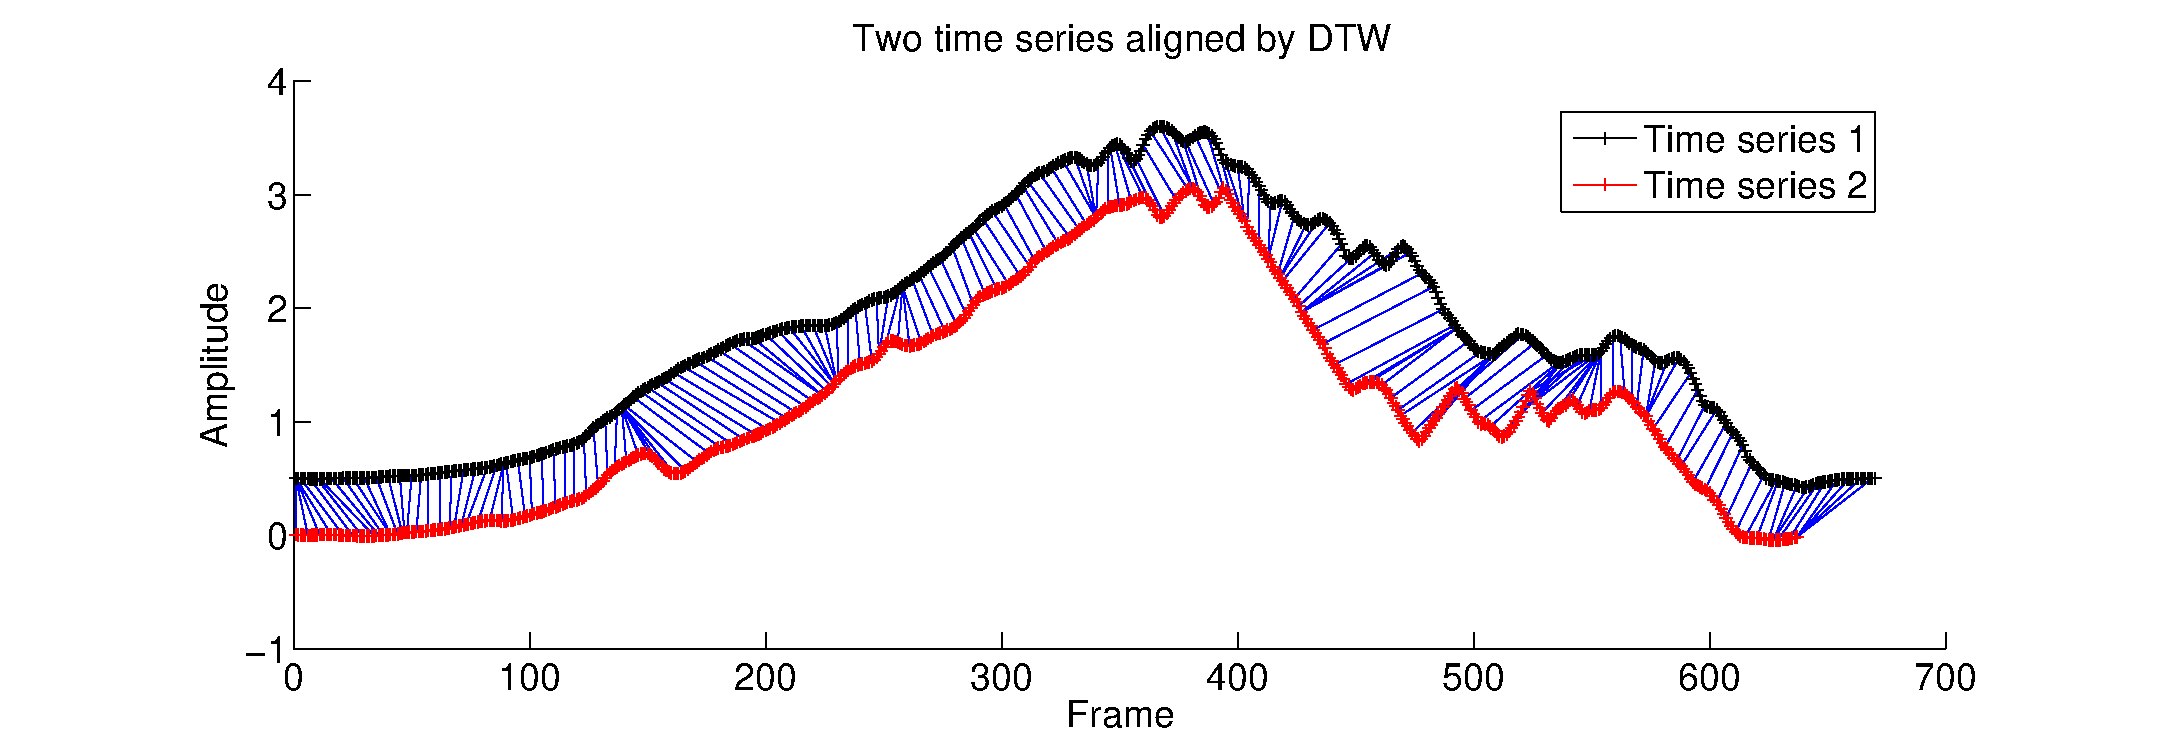
\includegraphics[width=16cm]{./fig_cha4/alignDTW.eps}
  \caption{ \scriptsize{Two time series aligned by DTW. Red and black lines are the raw time series. The blue lines connect the matching points between them. DTW wrap the two time series non-linearly so that the time independence similarity can be measured. The time series 1 is moved up by 0.5 for display reasons.}
}
\label{fig:alignDTW}
\end{figure}



\paragraph{Grouping data} ~\\
Two of the most common clustering methods are k-means clustering and hierarchical clustering. K-means is a centroid based grouping method. Given the number of clusters k, it finds a way to group the data such that the sum of the distance from each point to its belonging group center is minimized. Hierarchical clustering is a connectivity based method. There are two types of hierarchical clustering methods: agglomerative and divisive. Here we focus on the agglomerative method as it is more widely used. The hierarchical clustering method groups similar data iteratively. At the beginning each data point is a single cluster. In each iteration, two most similar clusters are merged to one. This step repeats until a stop criteria is satisfied or all data is merged to one cluster. Usually the merges are done in a greedy manner and hence no optimization is needed. Figure~\ref{fig:hcluster} illustrates the principle of hierarchical clustering. This clustering algorithm does not need to know the number of clusters in advance.

%% ------------ Hierarchical clustering -----------
In our case, the number of clusters is an unknown variable. Therefore we use the hierarchical (agglomerative) clustering method~\cite{willett1988recent} to group our data. The similarity (distance) between each pair of time series is computed by DTW. This produces a distance matrix. Each element in the matrix is the distance between two time series a and b, where a and b are the row and column index of the element. At the beginning of clustering, each time series is a single cluster. The distance between each cluster is read from the distance matrix. After one iteration, clusters are merged and most new clusters contain more than one time series. The distance between the new clusters is computed by the average distance between a member of one cluster to a member of the other cluster (average linkage).

\begin{figure}
  \centering
   \includegraphics[width=12cm]{./fig_cha4/hierarchicalclustering.pdf}
  \caption{ \scriptsize{A sketch of the hierarchical agglomerative clustering method. The nearest two clusters are grouped into one at each iteration until a single cluster is formed.}
}
\label{fig:hcluster}
\end{figure}

Our hierarchical clustering method has one more constraint: the threshold of distance. Two clusters can be merged into one only when their distance is smaller than the threshold. This threshold is set by the variance of the data from the same setup. As mentioned above (Section~\ref{cha4:sec2:demo}), a task is demonstrated a few times under the same setup. These demonstrations are presumed to be handled with the same strategy and hence belong to the same cluster. The variance of these demonstrations gives a reference of the variance of a cluster. The largest variance, across the variance of all setups, is used as the threshold for the clustering. Our clustering method is described as follow:

\begin{enumerate}
\item At the beginning, each single time series is considered to be one cluster.
\item Compute the distances between each pair of clusters.
\item Starting from the first cluster, find its nearest cluster.We define the distance between two clusters to be the average distance across all the time series pairs in each cluster.If the distance to the nearest cluster is smaller than the threshold, merge these two clusters. Otherwise leave these two separated.
\item Move to the next cluster. Repeat the last step for the rest of the clusters.
\item A new set of clusters will have been formed by the last few steps. Move to the next level of the hierarchy and repeat the step 2 to 4 until no new clusters can be formed, i.e. no pairs of clusters have distance smaller than the threshold.
\end{enumerate}

Pseudocode of the complete algorithm is shown in Algorithm~\ref{code:cluster}.

\begin{algorithm}
  \caption{Agglomerative Hierarchical Clustering}
  \begin{algorithmic}[1]
%    \Require{$x$ and $y$ are packed strings of equal length $n$}
%    \Statex Init();
    \State Init(): Make each time series a cluster; set the threshold\;
    \State $mergeable$ = true\;
    \Function{Merge}{all clusters, distance matrix} %      \Comment{$\oplus$: bit}
    \While{mergeable is true}
      \State $mergeable$ = false\;
      \For{each cluster}
        \State $ClusterA$ = current cluster\;
        \State $ClusterB$ = nearest neighbor of $ClusterA$\;
        \If{distance($ClusterA, ClusterB$) $<$ clustering threshold}
            \State Merge $ClusterB$ into $ClusterA$\;
            \State $mergeable$ = true\;
        \EndIf
      \EndFor
      %\State \Return{$\delta$}
    \EndWhile
    \EndFunction
  \end{algorithmic}
  \label{code:cluster}
\end{algorithm}

% --------- Number of cluster -----------
When the clusters cannot be merged further, we define the number of modules for this task: it is the number of the remaining
clusters. Each cluster is used as a module. The pattern of the data in a cluster represents a strategy for handling a specific task context.



\subsubsection{Learning Internal Models for Each Module}
\label{cha4:sec2:learn:model}

%%%%%%%%%%  TODO: MOSAIC
After identifying the number of modules and the data assigned to each, we build models for each module from its associated data. In this section, we explain the way we encode human manipulation strategy using machine learning to build the modules.

We aim to build a model that closely emulates the human motor strategy
in order to make the best use of the human data. Evidences of neuroscience suggest that human develop internal model for motor control, so as to estimate the outcome of a motor command. The use of internal model speed up the human correction and reaction in motor control. One hypothesis of the internal model is MOSAIC, which is a multiple modular model composed by a couple of pairs of forward model and inverse model. We build our control strategy based on this hypothesis.

\paragraph{MOSAIC} ~\\
MOSAIC~(MOdular Selection And
Identification for Control)~\citep{haruno2001mosaic} is a paradigm of multiple-module control,
where each module is composed of a forward model and an inverse
model. The forward models are responsible for estimating the task
context in real time, and the inverse models are used to generate
appropriate motor commands for the current context. The inverse models
are weighted by the accuracy of the estimations of their corresponding
forward models. The final motor command is the linear combination of
the commands factored by their weights.

We take the paradigm of MOSAIC but implement the modular model in our own manner. In earlier work, \citet{wolpert1998multiple} used
Artificial Neural Network (ANN) to encode the internal models,
i.e. the forward models and the inverse models. The variance of a
forward model, which decides how much the multiple modules
collaborate, has to be manually tuned. MOSAIC addresses this
hand-tuning problem by modeling the transition between modules using a Hidden Markov Model~(HMM) and optimizing the variance with the
Expectation Maximization~(EM) algorithm~\citep{haruno2001mosaic}. In
this method the forward models are approximated by linear systems. In order to solve the hand tuning problem of the variance but without restricting the complexity of the internal models, we encode our internal models with
Gaussian Mixture Models~(GMM)~\citep{cohn1996active}.

%During demonstrations, we constantly acquire the object displacements and the force and torque applied by the demonstrator. The demonstrator is the only source of exerted force and torque in the system. The relationship between the exerted force and torque and their resulting object displacement shows the dynamic characteristics of the task.

%GMM
\paragraph{Gaussian Mixture Model} ~\\
We model the correlation of the force and the displacement with
GMM. The task dynamics is hence encoded as a joint distribution of the object status displacement $s$ and the action $a$ taken by the human, $p(s,a,{\mid}{\Omega})$. In our experiment, $s$ is the one-dimensional angular displacement of the cap, and $a$ is the one-dimensional exerted torque and grip force.
Modeling a distribution by GMM allows us to capture the nonlinearity in the data, and also to compute the likelihood of a query data point in the model. This provides a good estimation of the reliability of the module in the current task context, which is crucial in choosing the correct modules for control  (discussed in Section~\ref{cha4:sec2:control:rf}).
Further, as a generative model GMM is able to
generate new data from the model, that is it allows us to generate motor commands. This is done by the {\em Gaussian Mixture Regression} (GMR). The general mathematical expression of GMM is explained in the previous chapter section~\ref{cha3:sec2:learn}. 

%\begin{table}
%\caption{Encoding process of GMM and computation process of GMR}
%    \colorbox{light-gray}{
%        \begin{minipage}[t]{1\textwidth}
%
%          With a Gaussian Mixture Model (GMM), the joint distribution
%          $\Omega$ of a set of variables $\{\eta\}$ is expressed as a
%          sum of $N$ Gaussian components:
%           \begin{equation}
%           \begin{split}
%            p\left(\eta\mid\Omega\right) = \sum_{n=1}^N \pi_n p\left(\eta\mid\mu_n,\Sigma_n\right) \\
%            = \sum_{n=1}^N \pi_n \frac{1}{\sqrt{\left(2\pi\right)^D \mid\Sigma_n\mid }} e^{-\frac{1}{2}\left(\eta-\mu_n\right)^{\top} \Sigma^{-1}_n \left(\eta-\mu_n\right)}
%           \end{split}
%           \end{equation}
%           where $\pi_n$ is the prior of the $n^{th}$ Gaussian component
%           and the ${\mu}_n$, ${\Sigma}_n$ the corresponding mean and
%           covariance, and $D$ the number of variables.
%
%
%            %% GMR:
%            Gaussian Mixture Regression (GMR) allows us to estimate the conditional expectation value of a variable $\eta^e$ given a query point $\eta^q$ where $\{\eta\} = \{\eta^q, \eta^e\}$. To compute this expectation value, first we define:
%            \begin{equation}
%            {
%             {\mu}_{n} = \begin{pmatrix} {\mu}_{n}^q    \\
%                                         {\mu}_{n}^e
%                         \end{pmatrix}
%            }
%%            \end{equation}
%%            \begin{equation}
%            \hspace{1cm}
%            {
%            {\Sigma}_{n} =  \begin{pmatrix} {\Sigma}_{n}^{qq}  & {\Sigma}_{n}^{qe}  \\
%                                            {\Sigma}_{n}^{eq} & {\Sigma}_{n}^{ee}
%                            \end{pmatrix}
%            }
%            \end{equation}
%
%            Secondly we compute the expected distribution of $\eta^e$ from the $n-th$ component:
%
%            \begin{equation}
%            {
%            \hat{\mu}_{n} = {\mu}_{n}^e + \Sigma_{n}^{eq}({\Sigma}_{n}^{qq})^{-1}(\eta^q-{\mu}_{n}^e)
%            }
%            \end{equation}
%
%            \begin{equation}
%            {
%            \hat{\Sigma}_{n} = {\Sigma}_{n}^{ee} - {\Sigma}_{n}^{eq}({\Sigma}_{n}^{qq})^{-1}{\Sigma}_{n}^{qe}
%            }
%            \end{equation}
%
%
%            Finally, all the $N$ Gaussian components are taken into
%            account, and the expectation value of variable $\eta^e$ is
%            computed as the mean $\hat{\mu}^e$ with the covariance
%            $\hat{\Sigma}^{ee}$:
%
%            \begin{equation}
%            {
%            \hat{\mu}^{e} = \sum_{n=1}^N{\beta_n}\hat{\mu}_{n}
%            }
%%            \end{equation}
%%            \begin{equation}
%            \hspace{1cm}
%            {
%            \hat{\Sigma}^{ee} = \sum_{n=1}^N{\beta_n}^2\hat{\Sigma}_{n}
%            }
%            \end{equation}
%
%            where
%            \begin{equation}
%            {
%            \beta_n = \frac{\pi_{n}p(q|{\mu}_{n}^q,{\Sigma}_{n}^{qq})}
%            {\sum_{n=1}^N{\pi_n}p(q|{\mu}_{n}^q,{\Sigma}_{n}^{qq})}
%            }
%            \end{equation}
%
%            Note that in a multiple module model, different module may have different number of Gaussian components.
%        \end{minipage}
%    }
%
%\label{tab:GMM}
%\end{table}



\paragraph{Internal Models}


%A forward model is held to anticipate the outcome of the motor command, while an inverse model is held to generate motor commands to take the current system state to the next state. The discrepancy between the anticipation of the forward model and the actual feedback is used to correct the motor command generated from the inverse model (Section~\ref{sec:rf}). Figure~\ref{fig:control} shows the basic control flow of a forward-inverse model pair.
As mentioned above, the internal models we are using here are the forward model and the inverse model.
A forward model is held to anticipate the outcome of the motor command, while an inverse model is held to generate motor commands to take the current system state to the next state. The discrepancy between the anticipation of the forward model and the actual feedback is used to correct the motor command generated from the inverse model (Section~\ref{cha4:sec2:control:rf}). Figure~\ref{fig:control} shows the basic control flow of a forward-inverse model pair.

\begin{figure}
  \centering
      \subfloat[\scriptsize{}]{\includegraphics[width=12cm]{./fig_cha4/control_1_2.pdf}}
      \vspace{0.5cm}
      \subfloat[\scriptsize{}]{\includegraphics[width=12cm]{./fig_cha4/control_3_2.pdf}}
      \caption{ \scriptsize{Control flow diagram of forward-inverse
          model in motor control. (a) System overview. Pairs of
          forward and inverse models work together to generate motor
          commands. The detailed mechanism inside the red box is shown
          underneath. (b) An example of a 3-module model. The forward
          models predict the current task context (s1, s2, s3) and
          estimate the accuracy of their prediction ($\lambda$1, $\lambda$2,
          $\lambda$3). These accuracy estimates are called ``Responsibility
          Factors'' as they also determine how much responsibility
          each inverse model should take in the final command. The
          inverse models generate commands (a1, a2, a3) and the final
          command is the summation of these, each weighted by its
          individual responsibility factor (a1$\lambda$1+a2$\lambda$2+a3$\lambda$3).  } }
\label{fig:control}
\end{figure}

% ----------- One model for both -------------
%The internal model ${\Omega})$ (forward model and inverse model) is encoded by the joint distributions of the variables, i.e. $p(s_t,s_{t+1},a_{t-1},a_t\mid{\Omega})$. This joint distribution encodes the forward model and the inverse model at the same time and both of their functionalities can be realized by the Gaussian Mixture Regression (GMR). For a given previous state and previous motor command, GMR provides a close-form solution to compute the anticipating state $s_t$, i.e. $p(s_{t+1}{\mid}s_{t},a_{t},{\Omega})$. For a given current state and desired state, we can compute the motor command using GMR, i.e. $p(a_t{\mid}s_t,s^{*}_{t+1},{\Omega_f})$. In some tasks, the initial status of the system remains unchanged for a certain time until the exert force or torque is big enough to change it. This will cause degeneracy in the inverse model. To solve this problem we include the previous motor command into the model, i.e. $p(a_t{\mid}s_t,s^{*}_{t+1},a_{t-1},{\Omega_f})$.

% --------- one model for each ----------
We encode the forward model $\Omega_F$ by the joint distributions of the current system state (object displacement), previous system state and the previous motor command, i.e. $p(s_t,s_{t-1},a_{t-1}\mid{\Omega_F})$, and similarly encode the inverse model $\Omega_I$ by the joint distributions of the current system state, the desired next system state, previous motor command and the current motor command, i.e. $p(s_t,s^{*}_{t+1},a_{t-1},a_t{\mid}{\Omega_I})$.
The previous motor command $a_{t-1}$ is necessary for the inverse
model. In some tasks, the system status can remains unchanged for a
certain period until the exerted force reaches a threshold to change
it. This will cause degeneracy in the inverse model; hence we
include the previous motor command in the model to tackle it.



% Non-linear, multi model. What to solve in multi model
%As discussed above, one of the characteristics of manipulation task is the changing kinematics and dynamics configuration.
%In different task contexts, the pattern of the correlation between the displacement and action may be different.

%By clustering the training data into different groups as discussed in Section~\ref{cha4:sec2:learn:cluster}, we are able to discover the number of different patterns, i.e. number of modules. We train one GMM on each of the modules to encode the different changing patterns of the task context.


% Learn system dynamics, impedance, admittance.

%Phases
%A single model is usually not enough to encode all these different configurations. Therefore we adopt a multiple modular approach to model the different environment. There are two key problems needed to be resolve in a multiple modular approach: how many models to build (Section~\ref{cluster}) and how to weight the models during the control process (Section~\ref{rf}).




\subsection{Multiple modular adaptive control and integration}
\label{cha4:sec2:control}
%% forward-inverse modeling
%%After clustering the data into different groups, we train each cluster with the GMM $p(X_T, X_{t+1}, U_{t-1}, U_t {\mid} {\Omega})$.
%We model each of the cluster to encode the human control policy under different dynamics.
%Neuroscientists suggested that human use a mixture of forward model and inverse model for motor control. The forward model
%With the learned multiple models, we adopt the MOSAIC~\cite{haruno2001mosaic} architecture to control the system. The basic concept of MOSAIC is that the human brain use multiple inverse models to control the system, which is augmented with a forward models. In human brain there exist multiple pairs of coupled forward and inverse models. The forward models estimate the reliability of the inverse model in the current context, and the final motor command is a linear combination of all the commands from the inverse models.
%In object manipulation, the system dynamics can be rapidly changing over time and we need more than one model to describe it. Our learnt multiple GMMs are used to describe the system in these different contents. First we need to infer the behavior of the system. Having deduced this information, we need to decide how to manipulate the system.

Once the number of modules is found and a pair of forward and inverse
models has been learnt for each, the modules can be used to compute
motor commands for task execution.  In our system of action selection,
this process of computing the command also computes a weight which
allows integration of the modules by simple summation.  We consider
the human motor system acted upon by motor command $a_t$ at time $t$
with current system status $s_t$. A function $f$ maps $a_t$ and $s_t$
to the system status at time $t+1$:

\begin{equation}
\label{e1}
s_{t+1} = f\left(s_t,a_t\right)
\end{equation}
The goal of the controller is to generate a motor command $a_t$ that
brings the current system status from $s_t$ to a desired state $s^*_{t+1}$:
\begin{equation}
\label{e2}
a_t = g\left({s^*_{t+1},s_t}\right)
\end{equation}

Equation~\ref{e1} represents the forward model and Equation~\ref{e2} represents the inverse model. In the modular approach, it takes two steps to compute the motor command $a_t$:
\begin{enumerate}
\item Anticipate the sensory output and compute the responsibility factor $\lambda_t$.
\item Compute motor command by each inverse model and compute the final motor command $a_t$.
\end{enumerate}


%\subsubsection{Anticipate sensory output by forward model}
%\label{cha4:sec2:control:forward}
%With the $k$-th forward model we can estimate the current status $\hat{s}_t$ by
%\begin{equation}
%\label{equ:e3}
%\hat{s}^k_{t} = E\left({s_{t-1}, a_{t-1} \mid \Omega^k_I}\right)
%\end{equation}

%and
%
%\begin{equation}
%\label{e4}
%u^i_t = E\left({x^*_{t+1},x_t, u^i_{t-1} \mid \Omega^i}\right)
%\end{equation}

%These two equations will be described later in details.

%This equation predicts the environment status based on the current observation and the prediction of the controller's influence on the system. The expectation values of the current system status of the $k$-th module is computed by the $Gaussian$ $Mixture$ $Regression$ (GMR). The computation is as follows.
%
%With the sensory input $\{s_{t-1},a_{t-1}\}$ as a query point $q$ we define:
%
%\begin{equation}
%{
% {\mu}_{q,n}^k = \begin{pmatrix} {\mu}_{s_{t-1},n}^k    \\
%                                        {\mu}_{a_{t-1},n}^k
%                        \end{pmatrix}
%}
%\end{equation}
%\begin{equation}
%{
%{\Sigma}_{qq,n}^k =  \begin{pmatrix} {\Sigma}_{s_{t-1}s_{t-1},n}^k  & {\Sigma}_{s_{t-1}{a_{t-1},n}}^k  \\
%                                            {\Sigma}_{{a_{t-1}}{s_{t-1}},n}^k  & {\Sigma}_{{a_{t-1}}{a_{t-1}},n}^k
%                            \end{pmatrix}
%}
%\end{equation}
%and GMR then uses:
%
%\begin{equation}
%{
%\hat{\mu}_{s_t,n}^k = {\mu}_{s_t,n}^k + \Sigma_{{s_t}q,n}^k({\Sigma}_{qq,n}^k)^{-1}(q-{\mu}_{q,n}^k)
%}
%\end{equation}
%
%\begin{equation}
%{
%\hat{\Sigma}_{{s_t}{s_t},n}^k = {\Sigma}_{{s_t}{s_t},n}^k - {\Sigma}_{{s_t}q,n}^k({\Sigma}_{qq,n}^k)^{-1}{\Sigma}_{q{s_t},n}^k
%}
%\end{equation}
%
%
%Finally, all the $N$ Gaussian components of the $k$-th module\footnote{Different modules may have different number of Gaussian components.} are taken into account and the current sensory data $\hat{s}_t$ is predicted as the mean $\hat{\mu}_{s_t}$ with the covariance $\hat{\Sigma}_{s_t,s_t}$ according to:
%
%\begin{equation}
%{
%\hat{\mu}_{s_t} = \sum_{n=1}^N{\beta_n(q)}\hat{\mu}_{s_t,n}^k
%}
%\end{equation}
%\begin{equation}
%{
%\hat{\Sigma}_{{s_t}{s_t},n} = \sum_{n=1}^N{\beta_n(q)}^2\hat{\Sigma}_{{s_t}{s_t},n}^k
%}
%\end{equation}
%where
%\begin{equation}
%{
%\beta_n(q) = \frac{p_{n}p(q|{\mu}_{q,n}^k,{\Sigma}_{qq,n}^k)}
%{\sum_{n=1}^N{p_n}p(q|{\mu}_{q,n}^k,{\Sigma}_{qq,n}^k)}
%}
%\end{equation}



\subsubsection{Weight modules by responsibility factor}
\label{cha4:sec2:control:rf}

In a modular approach, choosing the proper modules to control the
system at every time increment is a crucial step. For this we rely on
a system of {\em responsibility factors}, which act as the weights of
the inverse models. The responsibility factor is a measurement of the
reliability of using one module to represent the current system
context.

With the $k-{th}$ forward model we can anticipate the current state ${\hat{s}} ^k_t$ by using $GMR$ (explained in the previous chapter section~\ref{cha3:sec2:learn}):
\begin{equation}
\label{e3}
{\hat{s}} ^k_{t} = E\left({s_t {\mid} s_{t-1}, a_{t-1}, \Omega^k_F}\right)
\end{equation}

By comparing the anticipated current state ${\hat{s}} ^k_t$ with the
actual current state $s_t$ detected by the sensors, we can evaluate
how well the $k-{th}$ module represents the current system. The actual
current state, previous state and the previous motor command form a
data point $\eta_t$ = $\{s_t,s_{t-1},a_{t-1}\}$. As the forward models
are built as GMM, it is easy to compute the likelihood of one data
point belongs to a particular model (the $k-th$ forward model): $p(\eta_t {\mid}
\Omega_F^k)$. The discrepancy between $\hat{s}^k_t$ and $s_t$ is
embedded in this likelihood and hence in practice we only compute the
$p(\eta_t {\mid} \Omega_F^k)$ and skip ${\hat{s}} ^k_t$.  The
responsibility factor of the $k-{th}$ inverse model is the likelihood of
the data point $\eta_t$ belongs to the $k-{th}$ module, normalized by
the total sum:

\begin{equation}
\lambda^k_t = \frac{p(\eta_t {\mid} \Omega_F^k)}{\sum_{j=1}^{J}{p(\eta_t {\mid} \Omega_F^j)}}
\end{equation}
where $J$ is the number of modules~\footnote{In the case that the
  dominator is very close to zero, the whole control process will be
  terminated as it indicates that the model is used on a different
  task.}.  At every time step, we compute the responsibility factor
for each module. The final motor command at that time step is the
linear combination of the commands generated from each inverse model
multiplied by its respective responsibility factor.

\subsubsection{Generate motor command by Inverse Model}
\label{cha4:sec2:control:inverse}


The motor command $a^k_t$ for the $k^{th}$ inverse model is computed
by GMR with the steps explained in Section~\ref{cha3:sec2:learn}. At each time
step, the responsibility factors $\lambda^k_t$ weight its
corresponding inverse model: the higher the responsibility is, the
more responsibility the inverse model takes in the control. The final
motor command generated by this multiple model system is:

\begin{equation}
\label{e_mix}
a_t = \sum_{k=1}^K{\lambda_t^k a_t^k} = \sum_{k=1}^K{\lambda_t^k E\left({a_t \mid s^*_{t+1},s_t, a_{t-1}, \Omega^k_I}\right)}
\end{equation}
where $K$ is the number of modules.

These three steps are all computed with a close form solution. This ensures that this system can react quickly to the changes in the environment by adjusting the responsibility factor.



